\documentclass[11pt]{article}

\usepackage[margin=1.0in]{geometry}
\usepackage{url, enumitem}
\usepackage{amsfonts, amsmath, amsthm, amssymb,bbm}
\usepackage{listings}
\usepackage{hyperref}
\usepackage{float}

\hypersetup{
    colorlinks=true,
    linkcolor=blue,
    filecolor=magenta,      
    urlcolor=cyan,
}
 
\urlstyle{same}


\usepackage{color,soul}


\theoremstyle{definition}
\newtheorem{defn}{Definition}[section]
\theoremstyle{plain}
\usepackage[textsize=tiny]{todonotes}


\usepackage{proof}
\usepackage{bussproofs}

% Some useful macros.
\newcommand{\given}{\,|\,}
\newcommand{\R}{\mathbb{R}}
\newcommand{\C}{\mathbb{C}}
\newcommand{\E}{\mathbb{E}}
\newcommand{\var}{\text{var}}
\newcommand{\cov}{\text{cov}}
\newcommand{\p}{\partial}
\newcommand{\mba}{\mathbf{a}}
\newcommand{\mbb}{\mathbf{b}}
\newcommand{\mbx}{\mathbf{x}}
\newcommand{\mcX}{\mathcal{X}}
\newcommand{\mcY}{\mathcal{Y}}
\newcommand{\boldw}{\mathbf{w}}
\newcommand{\mbxt}{\tilde{\mathbf{x}}}
\newcommand{\Sigmat}{\tilde{\Sigma}}
\newcommand{\mbz}{\mathbf{z}}
\newcommand{\mbw}{\mathbf{w}}
\newcommand{\mcN}{\mathcal{N}}
\newcommand{\mcP}{\mathcal{P}}
\newcommand{\eps}{\epsilon}
\newcommand{\trans}{\intercal}
\newcommand{\Ut}{\tilde{U}}
\newcommand{\Beta}{\text{Beta}}
\newcommand{\Bernoulli}{\text{Bernoulli}}
\newcommand{\Elbo}{\text{ELBO}}
\newcommand{\KL}{\text{KL}}
\DeclareMathOperator*{\argmax}{arg\,max}
\DeclareMathOperator*{\argmin}{arg\,min}
\newcommand{\angstrom}{\textup{\AA}}
\renewcommand{\v}[1]{\mathbf{#1}}
\renewcommand{\b}[1]{\mathbb{#1}}

\hypersetup{
    colorlinks=true,
    linkcolor=blue,
    filecolor=magenta
    urlcolor=cyan,
}
\lstset{
    basicstyle=\ttfamily,
    mathescape
}


% Author: Mark Goldstein
% Date: Summer 2018
\begin{document}
\begin{center}
Auto Diff\\ 
Mark Goldstein
\end{center}


\section{Definition of Derivative}

\noindent The derivative $f^\prime x$ of a function $f: \b{R} \rightarrow \b{R}$
at a point $x$ (in the domain of $f)$ is the slope of the tangent line to $f$
at the point $x$, defined by:
$$ f^\prime x = \lim_{\epsilon \rightarrow 0} \frac{f(x+\epsilon) - f(x)}{\epsilon} $$

\noindent When $f$ is a scalar-valued function of a vector-valued argument, 
we use the notation of partial derivatives with respect to $n$ scalar components. 
If $f: \b{R}^n \rightarrow \b{R}$, then we have a vector with entries 
$\partial f / \partial x_j$ for $j \in \{1,...,n\}$
called the gradient vector and notated with $\nabla$:

$$ \nabla f = \Big( \frac{\partial f}{\partial x_1},...,\frac{\partial f}{\partial x_n} \Big )$$

\noindent When the codomain $\b{R}^m$ is non-scalar, we have a matrix $\v{J}$ (the Jacobian)
with $J_{ij} = \partial f_i / \partial x_j = \partial y_i / \partial x_j$ for 
$i \in \{1,...,m\}$, $j \in \{1,...,n\}$  where each $f_i$ is the projection of the $i^{th}$ 
scalar of the result of $f$. Here is the notation for evaluating the Jacobian at a 
particular point $\v{x}=\v{a}$:

\begin{figure}[H]
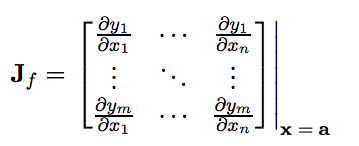
\includegraphics[width=8cm]{jacobian}
\centering
\end{figure}

\noindent The scalar chain rule for derivatives of compositions says:

\begin{align*}
    \frac{d}{dx}(f(x)+g(x)) &\rightarrow \frac{d}{dx}f(x) + \frac{d}{dx}g(x)\\
    \frac{d}{dx}(f(x)g(x)) &\rightarrow \Big(\frac{d}{dx} f(x) \Big)g(x) +
                                        f(x)\Big(\frac{d}{dx}g(x) \Big)
\end{align*}


\noindent The vector-valued chain rule says that when
$\v{x}$ is a vector, $\v{g}(x)$ is a vector-valued function of a vector argument, and
$f(\v{u})$ is a scalar-valued function of a vector-argument:

$$ \frac{\partial f \circ \v{g}}{\partial x_i} = 
\nabla f  \cdot \frac{\partial \v{g}}{\partial x_i} 
\quad \text{or, acting on x:} \quad
\frac{\partial f \circ \v{g}}{\partial x_i}\big( \v{x} \big) = 
\big(\nabla f\big) (\v{g}(\v{x}))  \cdot \frac{\partial \v{g}}{\partial x_i} \big( \v{x} \big)
$$

\noindent When $f$ is vector-to-vector this generalizes as:

$$ \frac{\partial \v{f} \circ \v{g}}{\partial x_i} = 
\sum_{\ell} \frac{\partial \v{f}}{\partial g_\ell}
\frac{\partial g_\ell}{\partial x_i} \quad \quad \text{each term $f$-dimensional, such derivative for each $x_i$} $$

\noindent This rule expresses the fact that a change in the $x_i$ 
direction may change all of $\{g_\ell\}$ and any of these changes may affect any
dimensions of $f$. Therefore, the derivatives of composed multivariate functions 
are chains of Jacobian matrix multiplications. Finally, note that one can obtain the directional
derivative of a scalar-valued function of $f$ with respect to its vector-valued argument
$\v{x}$ along a direction $\v{r}$ by performing a Jacobian-vector product (JVP) of
$\v{J}_f \cdot \v{r}$.

\newpage

\section{Automatic Differentiation}

\noindent Mainly following [Baydin et al 2018].
Methods for computing derivatives in computer programs can be classified into four categories:

\begin{enumerate}
    \item manually working out derivatives and coding them (error prone)
    \item numerical differentiation using finite difference approximations
          (highly inaccurate due to round-off and truncation errors, scales
          poorly for gradients with respect to millions of parameters)
    \item symbolic differentiation using expression manipulation in 
          computer algebra systems (results in complex, cryptic expressions,
          requires closed form expressions, e.g. no loops) 
    \item automatic differentiation (what this discussion is about)
\end{enumerate}

\noindent Automatic Differentiation (autodiff / AD) 
performs non-standard interpretation of a given computer program
by replacing the domain of the variables to incorporate derivative values
and redefining the semantics of the operators to propagate derivatives
per the chain rule of differential calculus. Some main points:

\begin{itemize}

\item Can be applied to regular code with minimal change,
allowing branching, loops, recursion. 

\item Numerical computations are compositions of finite set of base operations for 
which derivatives are known. These are combined through the chain rule to give derivatives of the compositions.
Operations include binary arithmetic operations, negation,
and transcendental functions such as the exponential, logarithm, and trig. functions.
Differentiation is not computable [Pour-El and Richards, 1978, 1983] for arbitrary functions, must use compositions.

\item Makes use of "evaluation traces": bookkeeping includes working variables that are assigned
the results of evaluating subexpressions. 

\item Because any numerical code will result in a numeric evaluation trace, 
code that loops and branches is differentiable: AD is blind with respect to any 
operation, including control flow statements, which do not directly alter numeric values.

\item AD has two main modes. Consider differentiating a function 
$f: \b{R}^n \rightarrow \b{R}^m$
    \begin{itemize}
        \item Forward Mode (or Forward
        accumulation mode, or tangent linear mode).
        This mode is better when $m > n$     

        \item Reverse Mode (or reverse accumulation mode,
        or adjoint linear mode or cotangent linear mode).
        Preferred when $n >> m$, which is often
        the case in machine learning, where we differentiate a \textit{scalar} 
        loss function with respect to \textit{millions} of parameters.
    \end{itemize}
\end{itemize}

\noindent First let's cover an evaluation trace example, cover dual numbers (important for AD) 
and then look at AD's two modes.

\newpage

\subsection{Evaluation Trace Conventions}

We will use Wengert Lists [Wengert, 1964] with three-part notation used by 
[Griewank and Walther 2008] where a function $f: \b{R}^n \rightarrow \b{R}^m$ 
is constructed issuing intermediate variables $v_i$ such that:

\begin{itemize}
    \item variables $v_{i-n} = x_i$ for $i=1,...,n$ are input variables
    \item variables $v_i$ for $i=1,...,l$ are working (intermediate) variables
    \item variables $y_{m-i} = v_{l-i}$ for $i=m-1,...,0$ are the output variables.
\end{itemize}

\noindent For our working example, consider $f(x_1,x_2) = \ln(x_1) + x_1x_2 - \sin(x_2)$. 
If we evaluate $f$ at input $(2,5)$, the evaluation trace (or in Forward-Mode AD terms,
the "forward primal trace") looks as follows:

\begin{figure}[H]
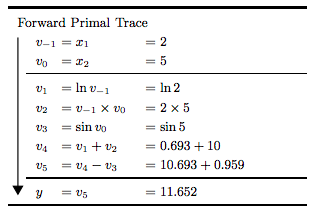
\includegraphics[width=8cm]{forward}
\centering
\end{figure}

\newpage

\subsection{Dual Numbers}

\noindent \textbf{Dual Numbers} are used to conveniently implement
one auto-differentiation approach (forward mode). We briefly review them
here, following [Mathoma 2016] and [Berland 2006]\\

\noindent Complex Numbers $\b{C}$:
\begin{itemize}
    \item numbers of form $a + bi$ where $i^2=-1$.
    \item multiplication rule: $(a+bi)(c+di) = ac - bd + (ad + bc)i$ 
          (consequence of $i^2=-1)$
\end{itemize}

\noindent Split Complex Numbers $\b{C}_s$:
\begin{itemize}
    \item numbers of form $a + bj$ where $j^2=1$ 
    \item multiplication rule: $(a + bj)(c + dj) = ac + bd + (ad + bc)j$ 
          (consequence of $j^2-1)$.
\end{itemize}

\noindent In both of the above: think about an imaginary unit, 
have it be equal to some number upon squaring, see what multiplication looks like.
How about $\epsilon$ such that $\epsilon^2=0$?\\

\noindent Dual Numbers $\b{D}$: 
\begin{itemize}
    \item numbers of form $a + b \epsilon$ where $\epsilon^2 = 0$
    \item multiplication: $(a + b \epsilon)(c + d \epsilon) = ac + (ad+bc)\epsilon$.
    \item Let's represent them as ordered pairs without reference to $\epsilon$.
    So $a + b\epsilon$ is written as $(a,b)$.
    \item multiplication rule becomes $(a,b)(c,d)=(ac,ad+bc)$. 
    \item Addition:$(a,b)+(c,d)=(a+c,b+d)$.
    \item $(0,1)(0,1)=(0,0)$. Two numbers not equal to $0$ multiply
    to $0$!
\end{itemize}

\newpage

\subsection{Using Dual Numbers for Differentiation}

Consider $f(x)=x^2$, $f: \b{R} \rightarrow \b{R}$. Let's expand this function to operate over duals, i.e. so $f: \b{D} \rightarrow \b{D}$.
Instead of evaluating $f(a)$ let's evaluate $f(a + 1 \epsilon)$:

$$f(a + 1\epsilon) = (a+1\epsilon)^2 = a^2 + 2a\epsilon + \epsilon^2 = a^2 + 2a \epsilon $$

\noindent where the last equality follows from $\epsilon^2=0$. 
Notice that $a^2$ is $f(a)$ and that $2a$ is $f^\prime(a)$. So $f(a+1\epsilon) = f(a) + f^\prime(a)\epsilon$ in this case.\\

\noindent Now consider polynomials over dual numbers. Let $P(x)= p_0 + p_1x + p_2x^2 +
... + p_n x^n$. Extend Extend $x$ to dual number $x + \dot{x}d$ where for now
assume $\dot{x}$ has no particular meaning and is just some number. Then
\begin{align*}
    P(x + \dot{x} \epsilon) &= 
        p_0 + p_1(x + \dot{x}\epsilon) + ... + p_n(x + \dot{x}\epsilon)^n\\
    &=  p_0 + p_1x + p_2x^2 + ... + p_n x^n \\
    &\phantom{a} + p_1 \dot{x} \epsilon + 2 p_2 x \dot{x} \epsilon + ... +
        n p_n x^{n-1} \dot{x} \epsilon \\
    &= P(x) + P^\prime(x) \dot{x} \epsilon    
\end{align*}

\noindent If you set $\dot{x}$ to $1$, then the coefficient of $\epsilon$ is
the derivative of $P$ evaluated at $x$. More generally,
$f(a + b \epsilon) = f(a) + f^\prime(a) b \epsilon$ 
($b$ doesn't have to be $1$). We now know that this holds for polynomials.
Similarly, one may derive

\begin{align*}
    \sin(x + \dot{x} \epsilon) &= \sin(x) + \cos(x) \dot{x} \epsilon\\
    \cos(x + \dot{x} \epsilon) &= \cos(x) - \sin(x) \dot{x} \epsilon\\
    e^{(x + \dot{x} \epsilon)} &= e^x + e^x \dot{x} \epsilon\\
    \log(x + \dot{x} \epsilon) &= \log(x) + \dot{x}\frac{1}{x} \epsilon, x \neq 0 \\
    \sqrt{x + \dot{x} \epsilon} &= \sqrt{x} + \dot{x} \frac{1}{2\sqrt{x}} \epsilon, x \neq 0
\end{align*}


\noindent This can be extended to functions of many variables
by introducing more dual components. For example, $f(x_1,x_2) = x_1 x_2 + \sin x_1$
extends to 
$$f(x_1 + \dot{x_1} \epsilon_1, x_2 + \dot{x_2} \epsilon_2) = 
(x_1 + \dot{x_1}\epsilon_1)(x_2 + \dot{x_2}\epsilon_2) + \sin(x_1 + \dot{x_1}\epsilon_1) =
x_1 x_2 + (x_2 + \cos(x_1))\dot{x_1}\epsilon_1 + x_1 \dot{x_2} \epsilon_2 $$
\noindent where the coefficients of $\epsilon_i$ are the partial derivatives with respect
to $x_i$ when $\dot{x_i}=1$. We now know that the derivative property holds
for many functions.

\newpage

\subsection{Forward Mode AD}

Consider again $f(x_1,x_2) = \ln(x_1) + x_1x_2 - \sin(x_2)$ whose evaluation trace is 
given above. For computing the derivative of $f$ with respect to $x_1$, we 
start by associating with each intermediate variable $v_i$ a derivative

$$ \dot{v_i} = \frac{\partial v_i}{\partial x_1} $$.

\noindent Applying chain rule to each elementary operation in the forward (primal)
trace, we generate the corresponding tangent (derivative) trace (right hand side of
augmented execution trace below). Evaluating the primals $v_i$ in alternation
with their corresponding tangents $\dot{v_i}$ gives us the required derivative
of the final variable $\dot{v_5} = \partial y / \partial x_1$:

\begin{figure}[H]
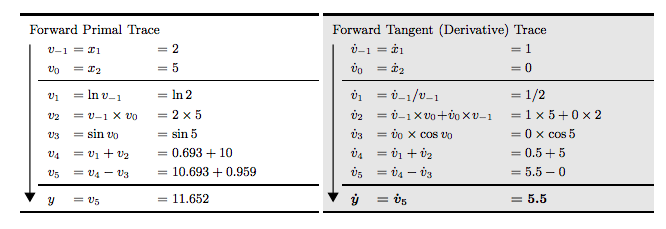
\includegraphics[width=12cm]{forward_dual}
\centering
\end{figure}


\noindent 
This generalizes to computing the Jacobian of a function $f: \b{R}^n \rightarrow \b{R}^m$
with $n$ independent input variables $x_i$ and $m$ dependent (output) variables $y_j$.
In this case, each forward pass of AD is initialized by setting only one of the variables
$\dot{x_i}=1$ and the rest to $0$. A run of the code with input $\v{x}=\v{a}$ computes

        $$ \dot{y_j} = \frac{\partial y_j}{\partial x_i} \rvert_{\v{x}=\v{a}}, 
            \quad j=1,...,m $$

\noindent and gives us one column of the Jacobian evaluated at the point $\v{a}$. The full
Jacobian can then be computed in $n$ evaluations. 
This also gives us the ability to compute Jacobian-vector products in a matrix-free way,
by initializing $\dot{\v{x}}=\v{r}$ and doing just one forward pass. When $f:\b{R}^n \rightarrow
\b{R}$ this gives us the directional derivative along $\v{r}$ (linear combination of partials)
$\nabla f^\top \cdot \v{r}$.\\

\noindent Forward mode can compute all derivatives $d y_j / dx$ for $f: \b{R} \rightarrow \b{R}^m$ in just one pass. Conversely, for $f: \b{R}^n \rightarrow \b{R}$ we need $n$ evaluations
to get the gradient vector

$$ \nabla f = \Big( \frac{\partial y}{\partial x_1},...,\frac{\partial y}{\partial x_n} \Big )$$

\noindent( a $1 \times n$ Jacobian built one column at a time with $n$ forward evaluations )

\newpage

\subsection{Implementation of Forward Mode with Dual Numbers}

\noindent Dual numbers are used in forward mode AD. The Dual Number addition
and multiplication rules mirror differentiation rules:
\begin{align*}
    (v + \dot{v} \epsilon) + (u + \dot{u} \epsilon) &= (v+u) (\dot{v}+\dot{u})\epsilon\\
    (v + \dot{v} \epsilon)(u + \dot{u}\epsilon) &= (vu) + (v \dot{u} + \dot{v} u )\epsilon
\end{align*}

\noindent If functions obey the following property:

$$ \texttt{Property 1.} f(a + b \epsilon) = f(a) + f^\prime(a) b \epsilon$$

\noindent then the chain rule works as expected on the dual number representation, which
can be seen by applying the property twice:

$$ f(g(v + \dot{v}\epsilon)) + f(g(v) + g^\prime(v) \dot{v} \epsilon) =
f(g(v)) + f^\prime(g(v))g^\prime(v) \dot{v} \epsilon $$

\noindent The coefficient on the right-hand side is exactly the derivative of the
composition of $f$ and $g$. 
This means that we can extract the derivative of a function by interpreting
any non-dual number $v$ as $(v + 0 \epsilon)$ and evaluating the function
in this non-standard way on an initial input with a coefficient of $1$ for $\epsilon$:

$$ \frac{d f(x)}{dx} \rvert_{x=v} = \texttt{Eps}(\texttt{dual-version}(f)(v+1\epsilon)) $$

\noindent where $\texttt{Eps}$ extracts $\epsilon's$ coefficient.
In practice, a function $f$ coded in a programming language would be fed
into an AD tool and augmented with extra code (or interpreted) to handle
dual operations so the function and its derivative are simultaneously computed.
Note that these tools require source code transformation or operator overloading.

\newpage

\subsection{Reverse Mode AD}

\noindent Reverse AD propagates derivatives backward from a given output. This
is done by complementing each intermediate variable $v_i$ with an adjoint

$$ \bar{v_i} = \frac{\partial y_j}{\partial v_i} $$

\noindent Derivatives are computed in the second phase of a two-phase process.
In the first phase, the original code is run \textit{forward}, populating intermediate
variables $v_i$ and recording the dependencies in the computational graph through
book-keeping. In the second phase, derivatives are calculated by propagating adjoints
$\bar{v_i}$ in reverse, from outputs to inputs.\\

\noindent Recall the example $y = f(x_1,x_2) = \ln(x_1) + x_1 x_2 - \sin(x_2)$.
Reverse Mode AD at work:
\begin{figure}[H]
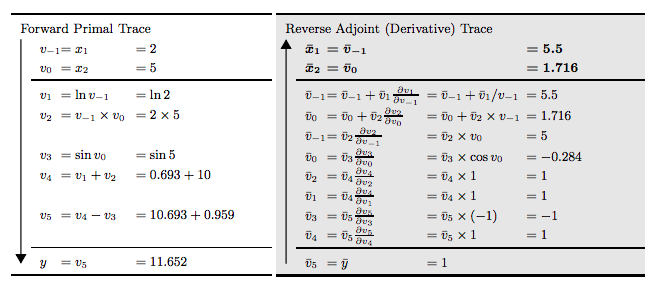
\includegraphics[width=14cm]{reverse}
\centering
\end{figure}

\noindent Consider $v_0$. It only affects $y$ through $v_2$ and $v_3$. Its
contribution to the change in $y$ is given by:

$$ \frac{\partial y}{\partial v_0} = \frac{\partial y}{\partial v_2} 
                                     \frac{\partial v_2}{\partial v_0} 
                                    +
                                     \frac{\partial y}{\partial v_3}
                                     \frac{\partial v_3}{\partial v_0}
\quad \text{or} \quad
\bar{v_0} = \bar{v_2} \frac{\partial v_2}{\partial v_0} 
             + \bar{v_3} \frac{\partial v_3}{\partial v_0} $$

\noindent In the table, this is computed in two steps:


$$ \bar{v_0} = \bar{v_3} \frac{\partial v_3}{\partial v_0} \quad \text{and} \quad
   \bar{v_0} = \bar{v_0} + \bar{v_2} \frac{\partial v_2}{\partial v_0} $$

\noindent which appear in the table lined up with the lines in the forward trace
from which these expressions originate. After the forward pass, we run
the reverse pass of the adjoints, starting with $\bar{v_5} = \bar{y} =
\frac{\partial y}{\partial y} = 1$. In the end we get derivatives
$\frac{\partial y}{\partial x_1} = \bar{x_1}$ and $\frac{\partial y}{\partial x_2} =
\bar{x_2}$ in just one reverse pass.\\

\noindent An advantage of reverse mode is that it is less costly to evaluate
than forward mode for functions with many inputs. In the extreme case,
$f: \b{R}^n \rightarrow \b{R}$, one application of reverse mode is sufficient
to compute the full gradient $\nabla f$, compared with the $n$ passes of
forward mode required. Because machine learning is focused on the
gradient of scalar-valued objectives with respect to large numbers of
parameters, this establishes the reverse mode as the mainstay technique.

\noindent Similar to matrix-free computation of JVP's with forward mode, reverse
mode can be used for computing the transposed Jacobian-vector product
$\v{J}_f^\top \v{r}$ by initializing the reverse phase with $\bar{\v{y}}=\v{r}$.

\noindent Note that reverse mode has storage requirements that in the worst case
grow in proportion to the number of operations in the function to be differentiated.

\subsection{Forward or Backward}

\begin{itemize}
    \item As mentioned, forward is better for the case of $\b{R} \rightarrow \b{R}^m$
    and reverse is better for the case of $\b{R}^n \rightarrow \b{R}$
    \item these are just two extremes: there is some optimal mix of approaches
          but it is NP-hard to find the best such approach.
\end{itemize}

\section{Gradient-Based Optimization}

\noindent Given an objective (loss) function $f(\v{w}): \b{R}^n \rightarrow \b{R}$
that one would like to minimize with respect to variable $\v{w}$,
one searches for (local) minimum $\v{w}^\star = \argmin_{\v{w}} f(\v{w})$ 
using an iterative steepest descent method. This is because usually
$f$ is complicated enough that one cannot simply set $\nabla f_{\v{w}} = 0$ and solve
for $\v{w}$, a method used to analytically find minima/maxima.\\

\noindent Steepest Descent methods pick the descent direction $\v{v}$ for which
the directional derivative $\nabla f^\top \v{v}$ is the most negative, subject
to $||\v{v}|| = 1$ for some choice of norm $||\cdot||$, and make updates to
$\v{w}$ by taking a step in that direction. When the norm is Euclidean, one
recovers the classical gradient descent algorithm, which uses
updates of the form $\Delta \v{w} = - \eta \nabla_{\v{w}} f$
where $\eta > 0$ is a step size.\\ 

\section{How ML Libraries work}

\noindent A typical machine learning library, PyTorch, works as follows.
A user specifies some variables $\v{w}_i$ to be optimized. Then the user
implements some ``forward" code that uses the $\v{w}_i$ to do something like make
a prediction. Following this, the user computes some loss function measuring
how well (how badly) they did and saves the result in a variable called \texttt{loss}. 
The goal is to tune the $\v{w}_i$ to minimize the value of $\texttt{loss}$.\\

\noindent During this computation, PyTorch builds a dependency graph of the 
expressions under the hood, where \texttt{loss} is the last vertex of the graph. 
A user then calls \texttt{loss.backward()} and Reverse-Mode AD uses the aforementioned
adjoints to compute the derivatives of the loss with respect to all of the variables
to be optimized $\v{w}_i$ and saves these derivatives in a $\texttt{.grad}$ field
for each such variable.\\

\noindent Finally, an optimizer (usually some object) that knows about the variables
to be optimized updates each one by reading the $\texttt{.grad}$ field and
applying something like gradient descent:

 $$\v{w}_i = \v{w}_i - \eta \v{w}_i\texttt{.grad}$$

\noindent perhaps with some additional tricks.\\

\noindent Actually, most practitioners and many researchers 
of machine learning exclusively use (and only know about) gradient descent,
and don't know that there are more general steepest descent methods 
(corresponding to different choices of norms). These alternatives are
better for optimizing certain kinds of problems, because those methods update the 
variables differently from just taking a step in the negative gradient direction. 
Rajesh has a paper on this. However, even when one knows about these alternatives,
they are hard to implement and experiment with because the setup described above is 
really intended for Eucidean-norm gradient descent.\\

\noindent One interesting research direction is how to make an auto-differentiation
+ optimization system that doesn't need separate implementations of descent
algorithms for each possible choice of norm. This might benefit from some
form of abstraction.

\section{Bayesian Probabilistic Modeling and Inference}

When introducing new models, machine learning researchers have spent considerable
effort on manual derivation of analytical derivatives to be used with
optimization algorithms (error prone and time consuming)\\

\noindent [ TODO ]

\section{Approximating Gradients of Expectations}

\noindent [ TODO ]

\section{Gradient Estimation Using Stochastic Computation Graphs}

\noindent [ TODO ] 

\newpage

\section{Citations}

\begin{itemize}
    
    \item  Baydin, Pearlmutter, Radul, Siskind
    Automatic Differentiation
    in Machine Learning: a Survey 2018
    \url{https://arxiv.org/pdf/1502.05767.pdf}

    \item The Simple Essence of Automatic Differentiation 2018
    CONAL ELLIOTT, \url{http://conal.net/papers/essence-of-ad/essence-of-ad-icfp.pdf}

    \item Good autodiff and dual number slides
    Havard Berland 2006
    \url{http://www.pvv.ntnu.no/~berland/resources/autodiff-triallecture.pdf}

    \item Marian Boykan Pour-El and Ian Richards. 1978. 
    Differentiability properties of computable functions - A summary. 
    Acta Cybernetica 4, 1 (1978), 
    \url{http://acta.bibl.u-szeged.hu/12271/1/cybernetica\_004\_fasc\_001\_123-125.pdf}

    \item Marian Boykan Pour-El and Ian Richards. 1983. 
    Computability and noncomputability in classical analysis. Transactions of
    the American Mathematical Society 275, 2 (1983)

    \item Mathoverflow about computability of differentiation: 
    ``John Myhill gave an example of a recursive function defined on a 
    compact interval and having a continuous derivative that is not recursive 
    [Michigan Math. J. 18 (1971), 97-98, MR0280373]. However, Pour-El and Richards 
    have shown that if a recursive function defined on a compact interval has a 
    continuous second derivative, then it has a recursive first derivative 
    [Computability and noncomputability in classical analysis, TAMS 275 (1983), 539-560"
    \url{https://mathoverflow.net/questions/35021/differentiability-of-computable-functions}

    \item Michael Spivak. 1965. Calculus on Manifolds: A Modern Approach to 
    Classical Theorems of Advanced Calculus. Addison-Wesley
    \url{http://strangebeautiful.com/other-texts/spivak-calc-manifolds.pdf}

    \item Gradient Estimation Using Stochastic Computation Graphs. 2016
    Schulman, Heess, Weber, Abbeel
    \url{https://arxiv.org/pdf/1506.05254.pdf}

    \item Robert E. Wengert. A simple automatic derivative evaluation program. 
    Communications of the ACM, 7:463–4, 1964.

    \item Andreas Griewank and Andrea Walther. Evaluating Derivatives: 
    Principles and Techniques of Algorithmic Differentiation. Society for 
    Industrial and Applied Mathematics, Philadelphia, 2008. doi: 10.1137/1.9780898717761.

    \item Mathoma (YouTube user). Dual Numbers Introduction. 2016.
    \url{https://www.youtube.com/watch?v=63dt-pSKlk0}

\end{itemize}

\end{document}



